\section{Draw your view of Pivotal's software development process }

\begin{figure}[H]
\centering
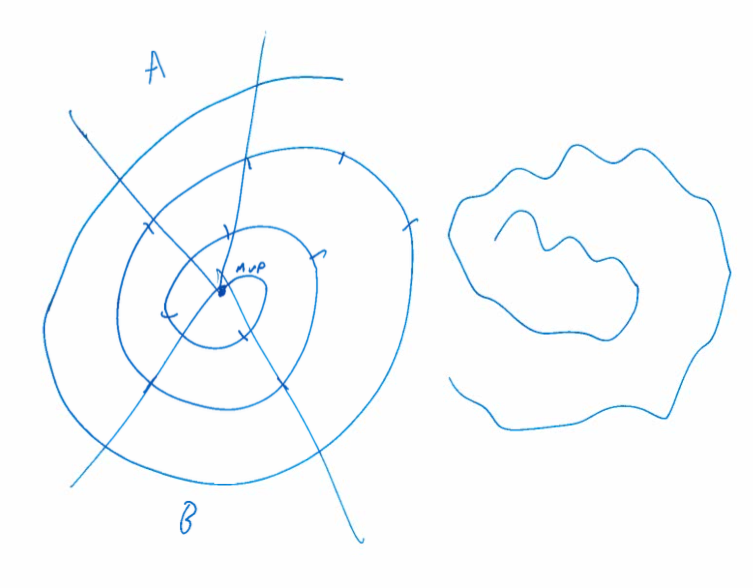
\includegraphics[width=6.5in]{interviews/drawings/2015_06_02.png}
\caption{\quotes{Interview 2: Product Manager's drawing of software development process}}
\end{figure}

\begin{figure}[H]
\centering
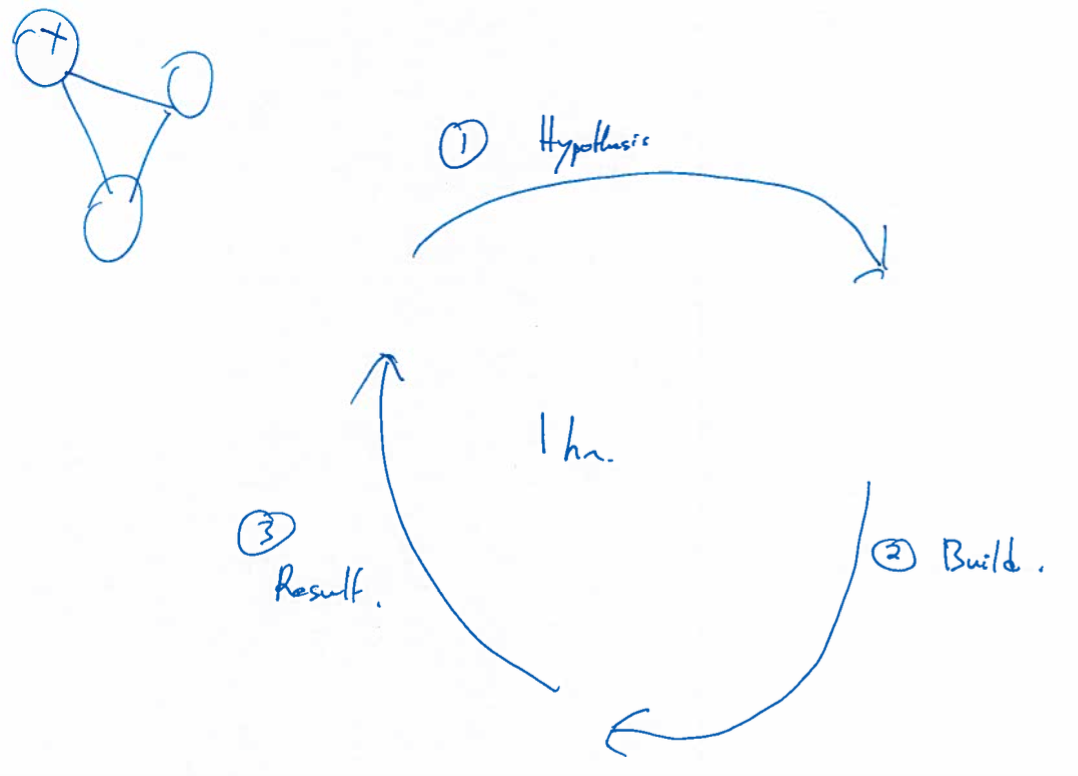
\includegraphics[width=6.5in]{interviews/drawings/2015_06_29a.png}
\caption{\quotes{Interview 3: Product Manager's drawing of software project workflow}}
\end{figure}

\textbf{Interviewee 3:} I try to first come up with some type of hypothesis that I want to test. Then, I'm going to build something that's going to test this, then I'm going to try to get a result. 

% \begin{figure}[H]
% \centering
% 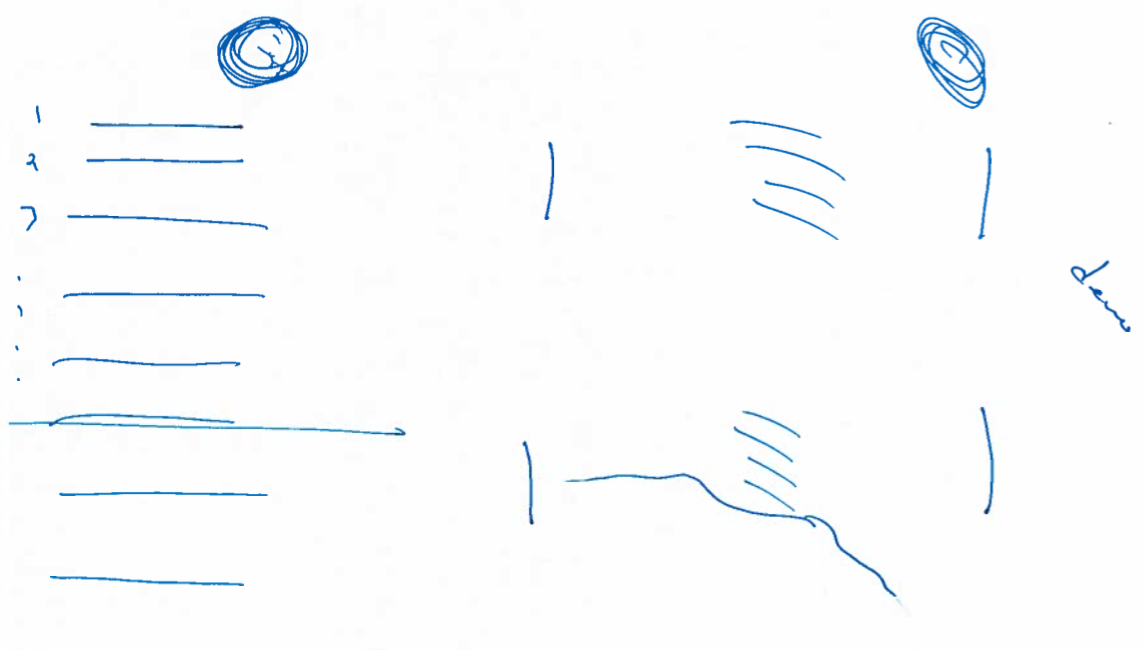
\includegraphics[width=6.5in]{interviews/drawings/2015_06_29b.png}
% \caption{\quotes{Interview 3:  Product Manager's drawing of software development process}}
% \end{figure}

\begin{figure}[H]
\centering
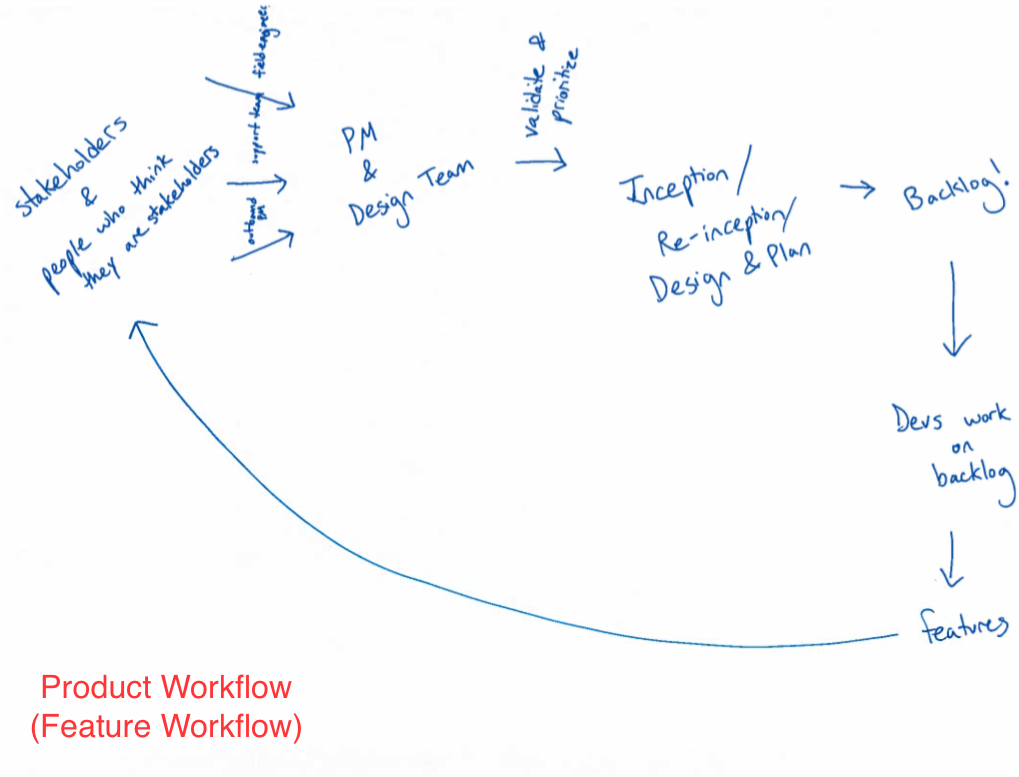
\includegraphics[width=6.5in]{interviews/drawings/2015_07_31a.png}
\caption{\quotes{Interview 5: Product Manager's drawing of software development process}}
\end{figure}

\begin{figure}[H]
\centering
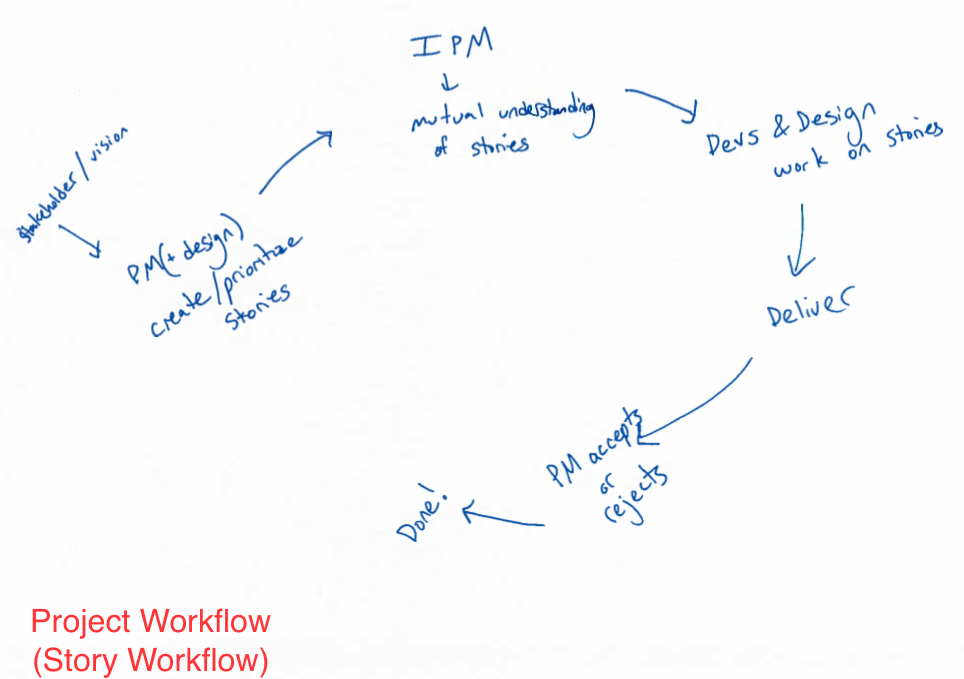
\includegraphics[width=6.5in]{interviews/drawings/2015_07_31b.png}
\caption{\quotes{Interview 5: Product Manager's drawing of software development process}}
\end{figure}

\begin{figure}[H]
\centering
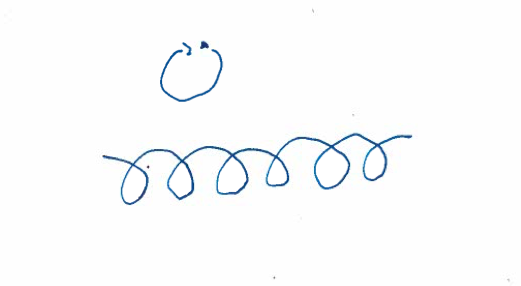
\includegraphics[width=6.5in]{interviews/drawings/2015_08_12_se.png}
\caption{\quotes{Interview 8: Software Engineer's drawing of software development process}}
\end{figure}

\textbf{Interviewee 8:} We iterate on stuff that we have a touch point and we're going to go away and do work and come back to that touch point. To me, it sort of looks more like a spring, you pull the slinky or you have a pig's tail that you stretched out. We are trying to do is orbit this idea of always working with each other. The red, green, refactor is a very tiny cycle that we do. We're trying to setup ourselves up, a check-in point where we can start somewhere and move a little bit and make sure we're okay and come back again and have another starting place and you can do that in 5 minutes with a test. Then you see us play that out at higher level of stories and then higher level again with our daily stand-ups, and higher level again with our retros and our check-ins there and higher level again with our inceptions. It's really about managing the feedback cycle or the check-in points to make sure that we're kind of all fluidly communicating about how we're affecting and doing things. Because the minute we stop communicating, is the minute we start to get off and be in the weeds somewhere.



\begin{figure}[H]
\centering
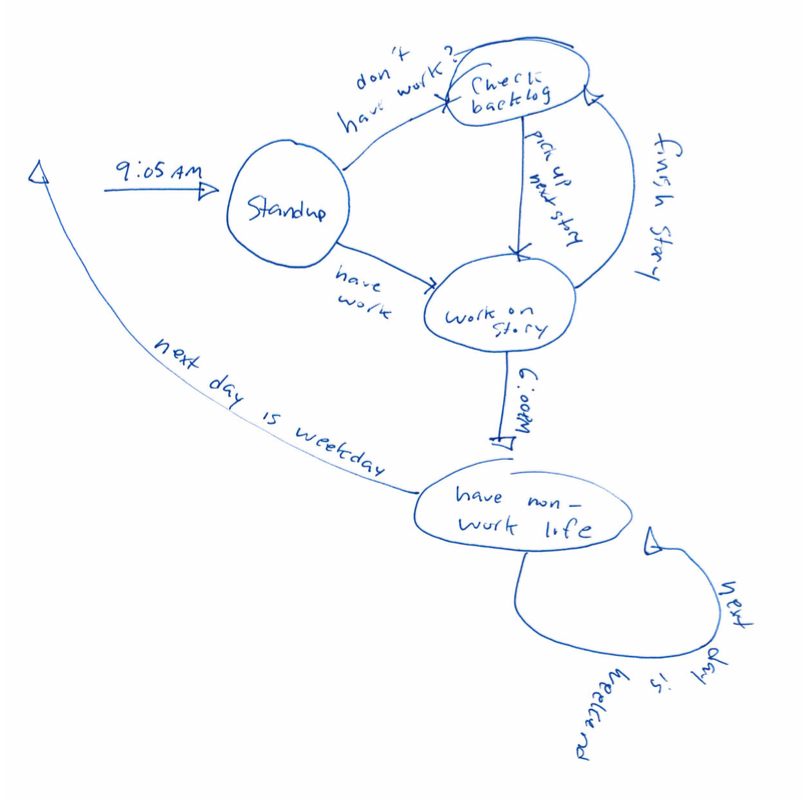
\includegraphics[width=6.5in]{interviews/drawings/2015_09_02.png}
\caption{\quotes{Interview 9: Software Engineer's drawing of project workflow}}
\end{figure}


% \begin{figure}[H]
% \centering
% 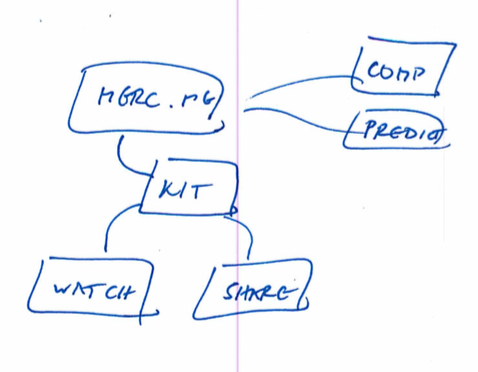
\includegraphics[width=6.5in]{interviews/drawings/2015_12_18a.png}
% \caption{\quotes{Software Engineer's drawing of software development?'}}
% \end{figure}

\begin{figure}[H]
\centering
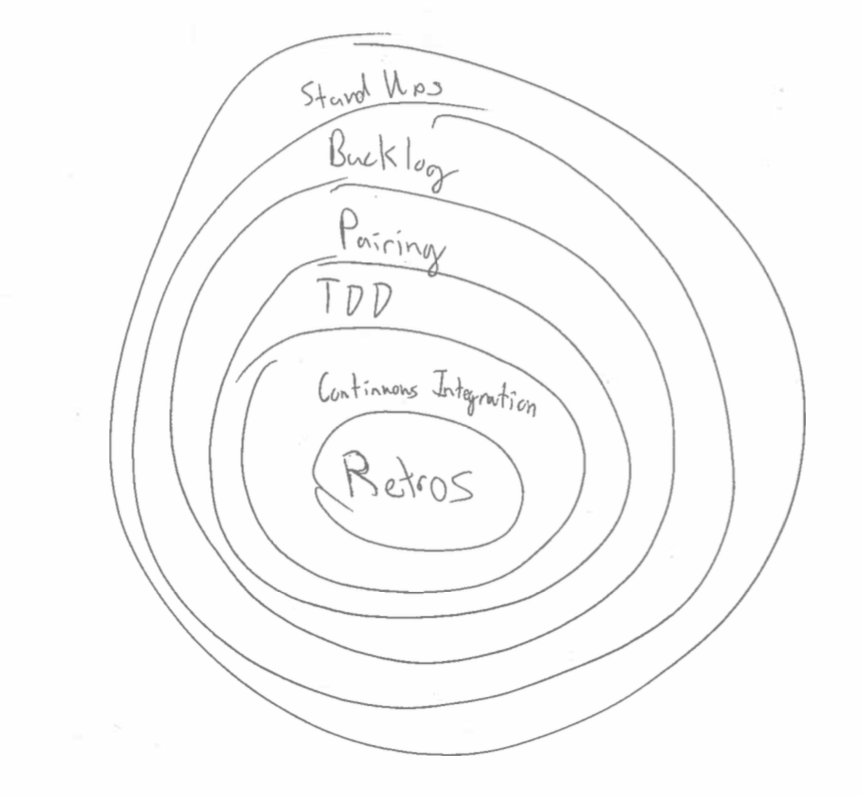
\includegraphics[width=5.5in]{interviews/drawings/2016_01_15.png}
\caption{\quotes{Interview 18: former software engineer's drawing for the Pivotal software development approach}}
\end{figure}

\textbf{Interviewee 18:} [The circles are arranged from an inner core practices to outer rings that are more negotiable.] These are the things I think are core to how Pivotal Labs does software development from the most important.  Basically, if some client wanted to drop things outside of it, this will be the order that I think we'd agree to have it be dropped.  I don't think we'd ever drop retros but I think we might drop the backlog or something that we probably still would.

\section{Draw how you feel about your current product?}

\begin{figure}[H]
\centering
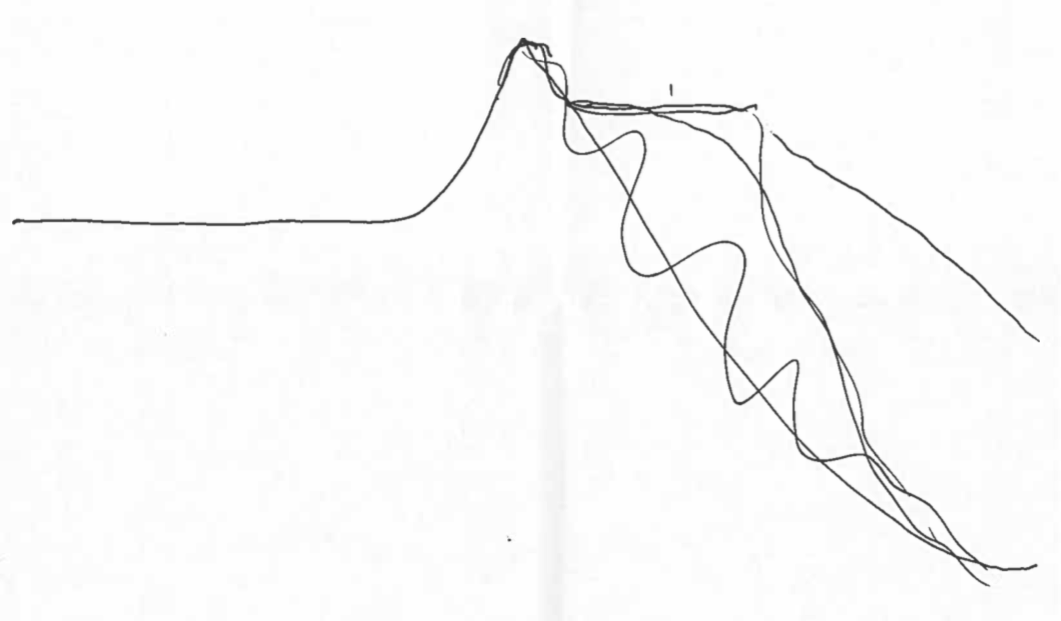
\includegraphics[width=6.5in]{interviews/drawings/2016_01_08_designer2.png}
\caption{\quotes{Interview 16: interaction designer's drawing for `how you feel about your current product?'}}
\end{figure}

\textbf{Interviewee 16:} The peak  was very like a successful moment for Pivotal. It's really cool to see how many people appreciated what we've done. Against all odds, we released this app. I felt proud to be on that team. \ldots 

[The graph goes down] as the design started getting cut. The only thing we're doing is bugs. We designed all these cool features that we're excited about. Almost none of them are getting into the app. It's been almost every week that a feature in the new design is no longer in [the release]. We don't need [what I worked on] anymore.  It feels very frustrating as a designer. I can't affect that that much.

\begin{figure}[H]
\centering
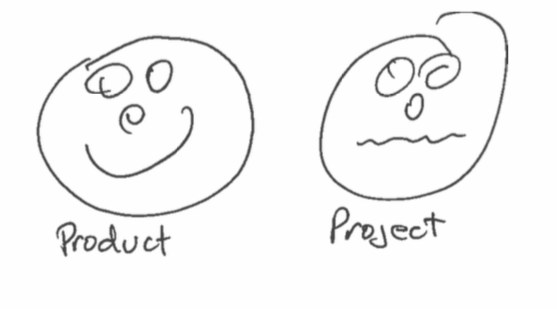
\includegraphics[width=6.5in]{interviews/drawings/2016_02_25.png}
\caption{\quotes{Interview 21: Product Manager's drawing for `how you feel about your current product'}}
\end{figure}

\section{Draw how you feel about the code}
\label{AppendixFeelAboutTheCode}

\begin{figure}[H]
\centering
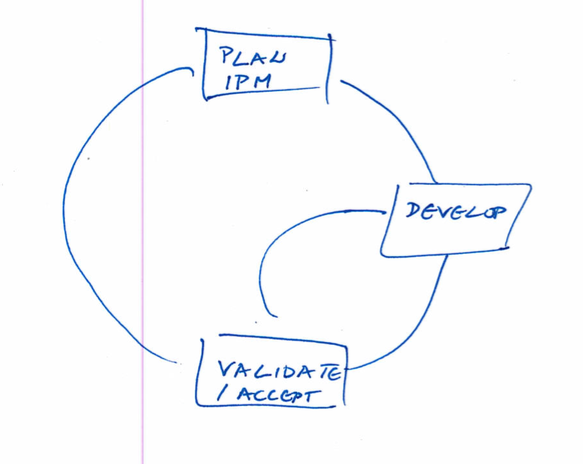
\includegraphics[width=6.5in]{interviews/drawings/2015_12_18b.png}
\caption{\quotes{Interview 14: Software Engineer's drawing for `how do you picture the code?'}}
\end{figure}


\begin{figure}[H]
\centering
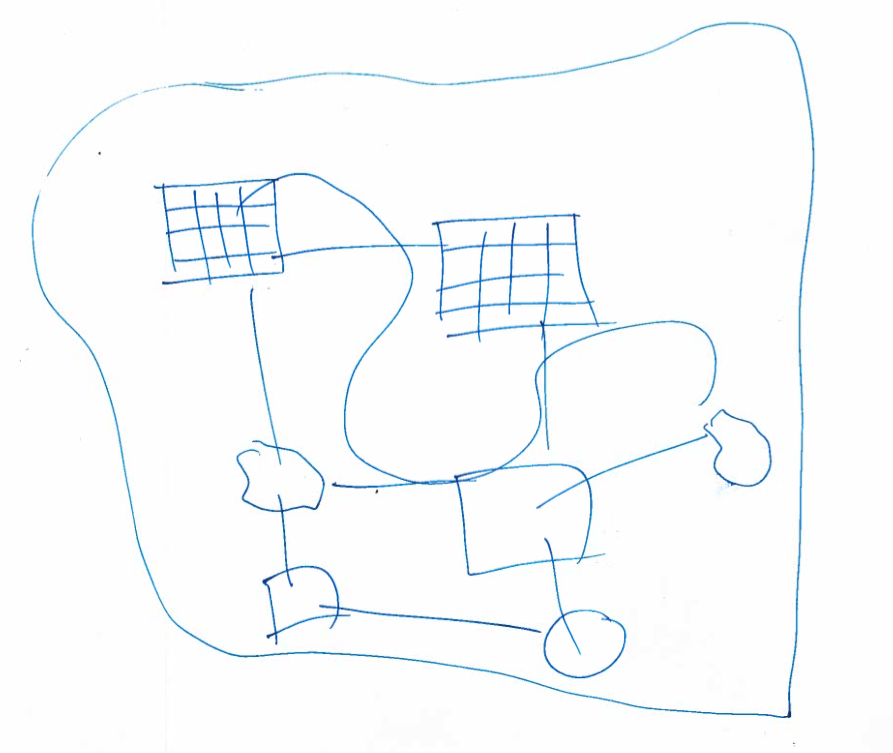
\includegraphics[width=6.5in]{interviews/drawings/2015_12_03.png}
\caption{\quotes{Interview 10 Software Engineer's drawing for `how you think of the code on this project?'}}
\end{figure}


\begin{figure}[H]
\centering
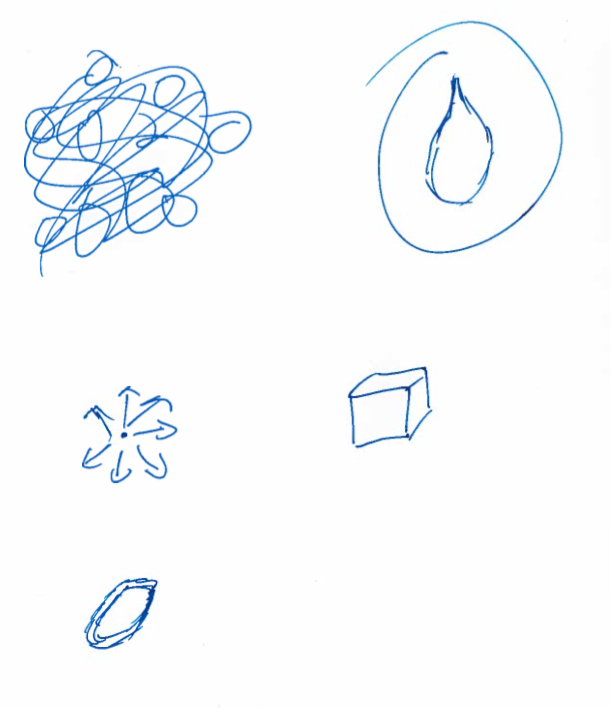
\includegraphics[width=6.5in]{interviews/drawings/2015_12_08.png}
\caption{\quotes{Interview 11: Software Engineer's drawing for `how you think about the code on this project?'}}
\end{figure}

\textbf{Interviewee 11:} It's kind of complicated. We have so many different pieces and this is what the connection feels like to me in my head where everything is jumbled together but at the same time, I do feel like the structure is clean but I'm having a hard time thinking of what to draw for like what represents clean. .  I'm just going to draw a water droplet to show that it looks clean.

It's more than just it's complicated, it's expanding a lot so in my head.  I'm thinking more like a big bang kind of thing where it starts out very small and now it just keeps expanding and growing and then we're adding a bunch of features. 

It's solid and clean. I feel like the project is very well tested so there's less chances of major breakings. It is solid. So I draw a rock cube.

Our codebase is pretty young, pretty flexible in ways that when we want to do refactors, it's not super complicated and not super hard to do. We are pretty good at like separating all the logic. It was really easy to do refactoring on the stuff that we want to do.  So, I guess it's pretty flexible of something flexible. So I draws a rubber band.

\begin{figure}[H]
\centering
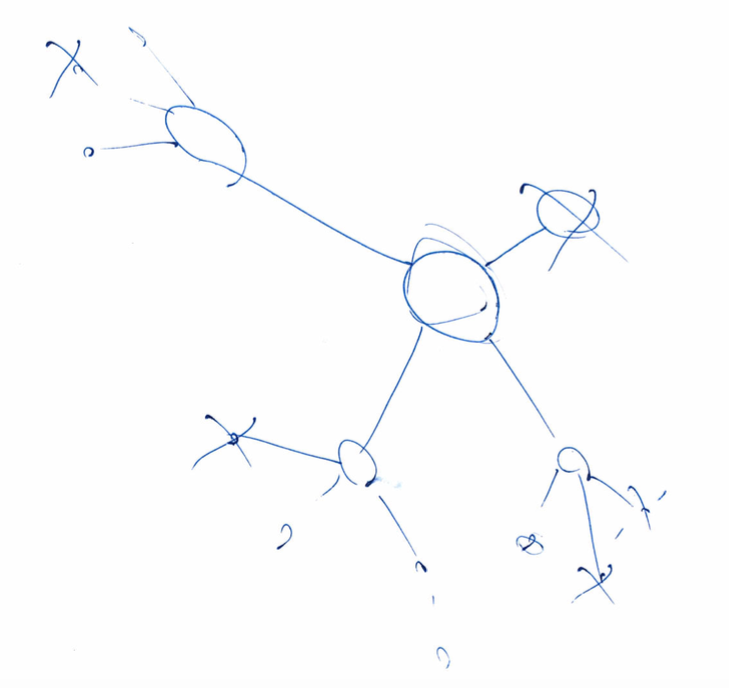
\includegraphics[width=6.5in]{interviews/drawings/2015_12_10.png}
\caption{\quotes{Interview 13: Software Engineer's drawing for `how you think about the code on this project?'}}
\end{figure}


\begin{figure}[H]
\centering
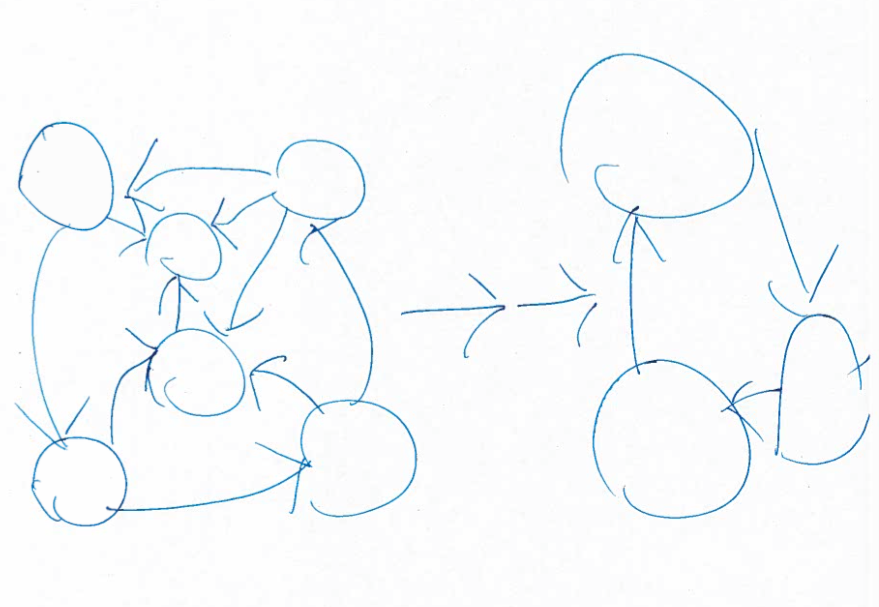
\includegraphics[width=6.5in]{interviews/drawings/2016_01_14.png}
\caption{\quotes{Interview 17: Software Engineer's drawing for `How you feel or how you think about the code'}}
\end{figure}


\begin{figure}[H]
\centering
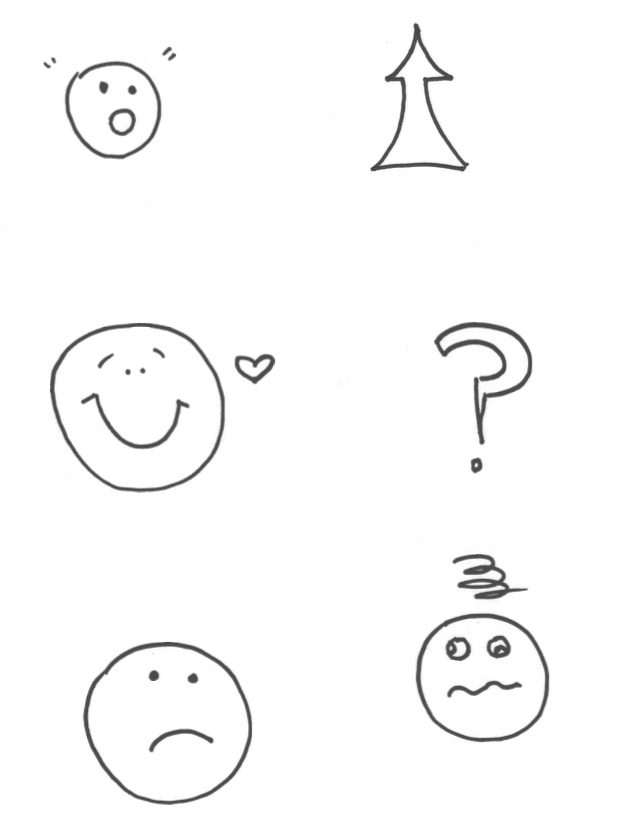
\includegraphics[width=6.5in]{interviews/drawings/2016_07_05a.png}
\caption{\quotes{Interview 25: Interaction Designer's drawing for `how you feel about your current product'}}
\end{figure}

\begin{figure}[H]
\centering
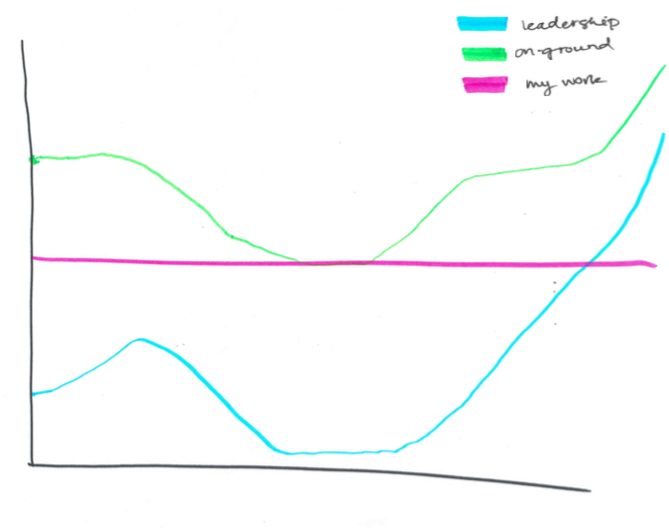
\includegraphics[width=6.5in]{interviews/drawings/2016_07_05b.png}
\caption{\quotes{Interview 25: Interaction Designer's drawing for `how you feel about your current product'}}
\end{figure}


\begin{figure}[H]
\centering
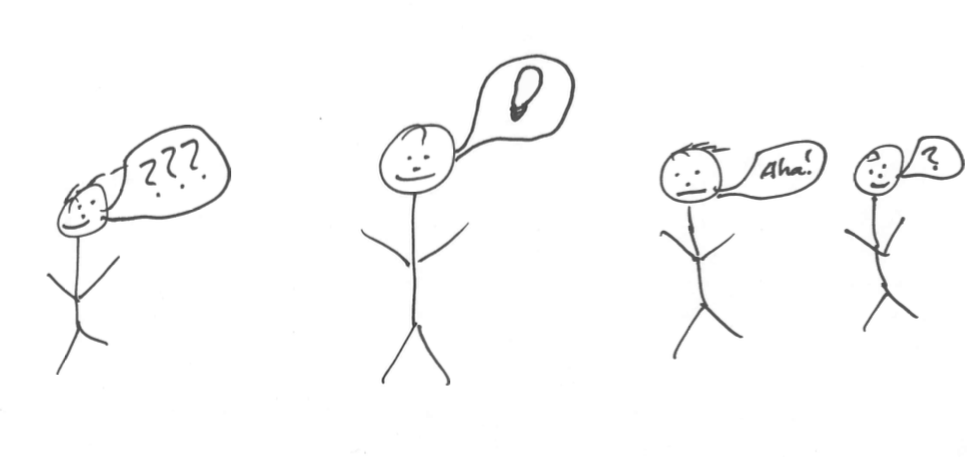
\includegraphics[width=6.5in]{interviews/drawings/2016_07_05_designer2.png}
\caption{\quotes{Interview 26: Interaction Designer's drawing for `How you feel or how you think about the code'}}
\end{figure}


\begin{figure}[H]
\centering
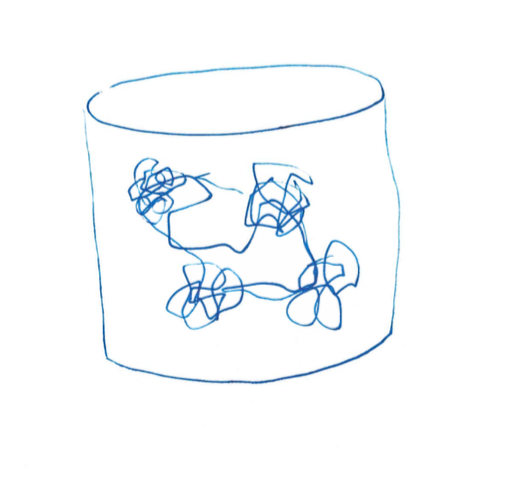
\includegraphics[width=6.5in]{interviews/drawings/2016_08_17.png}
\caption{\quotes{Interview 28: Software Engineer's drawing for `How you feel or how you think about the code'}}
\end{figure}

\begin{figure}[H]
\centering
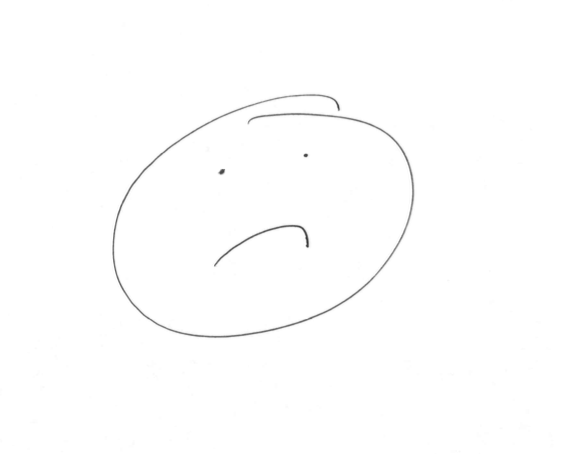
\includegraphics[width=6.5in]{interviews/drawings/2016_08_18.png}
\caption{\quotes{Interview 29: Software Engineer's drawing for `How you feel or how you think about the code'}}
\end{figure}

\begin{figure}[H]
\centering
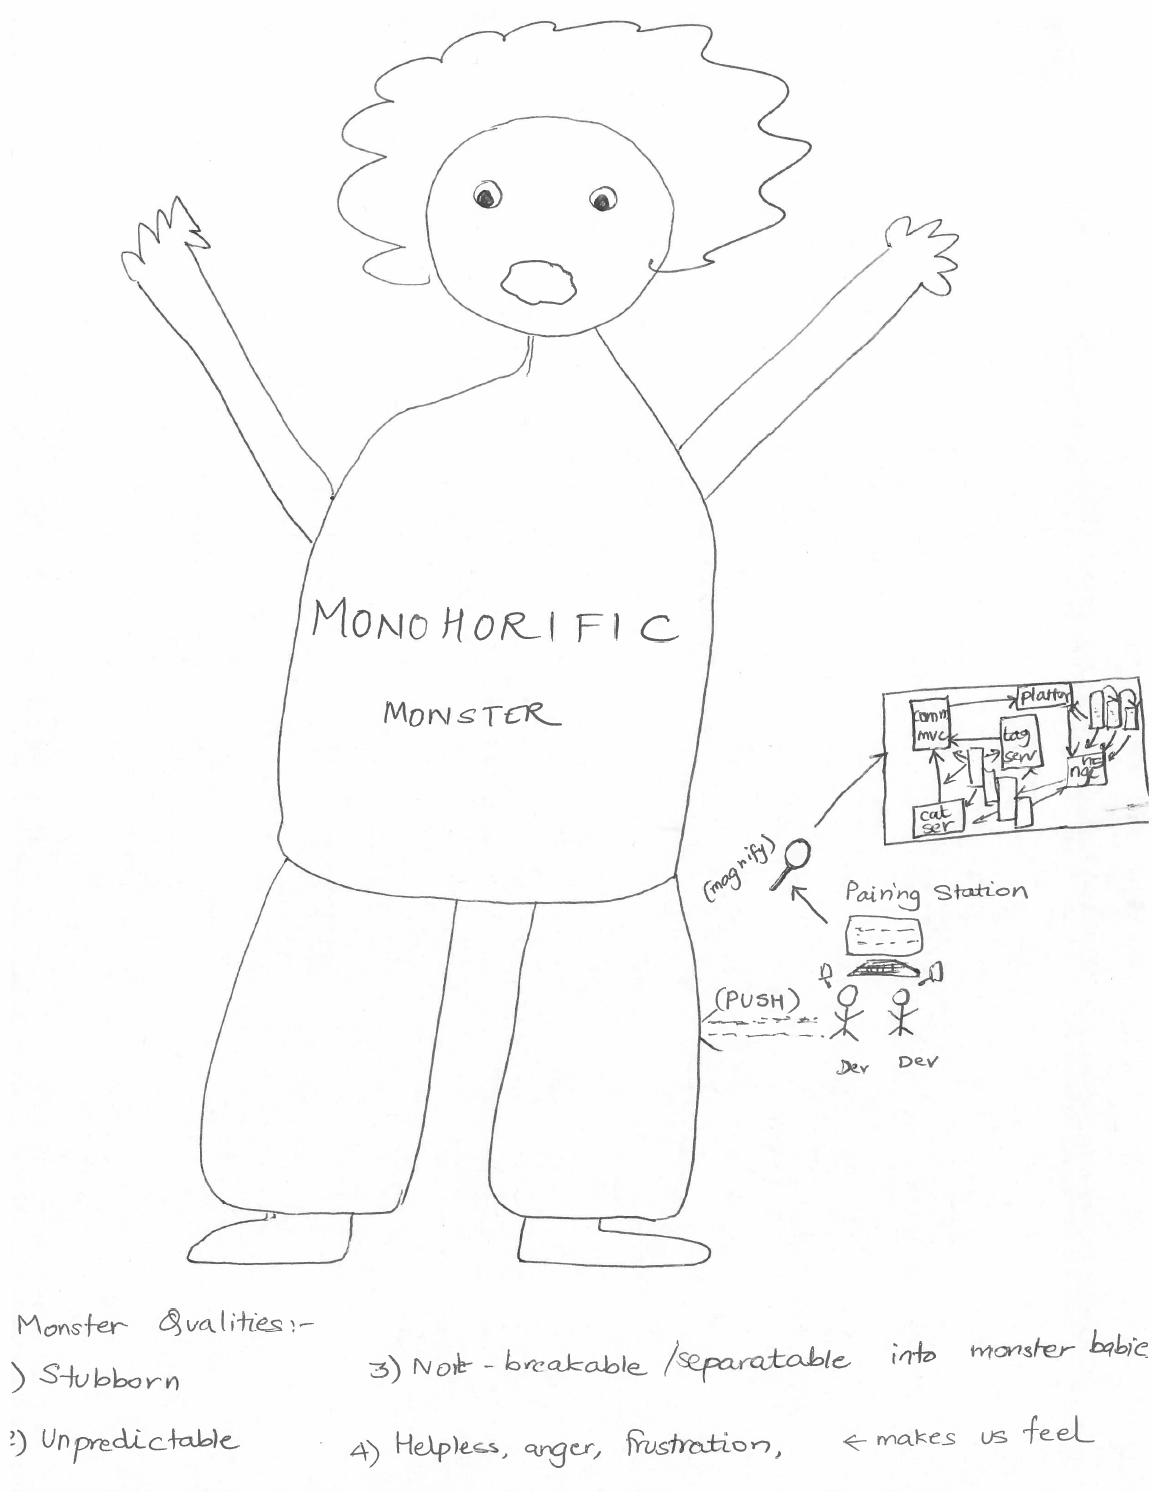
\includegraphics[width=6.5in]{interviews/drawings/2016_09_26.png}
\caption{\quotes{Interview 31: Software Engineer's drawing for `How you feel or how you think about the code'}}
\end{figure}

\begin{figure}[H]
\centering
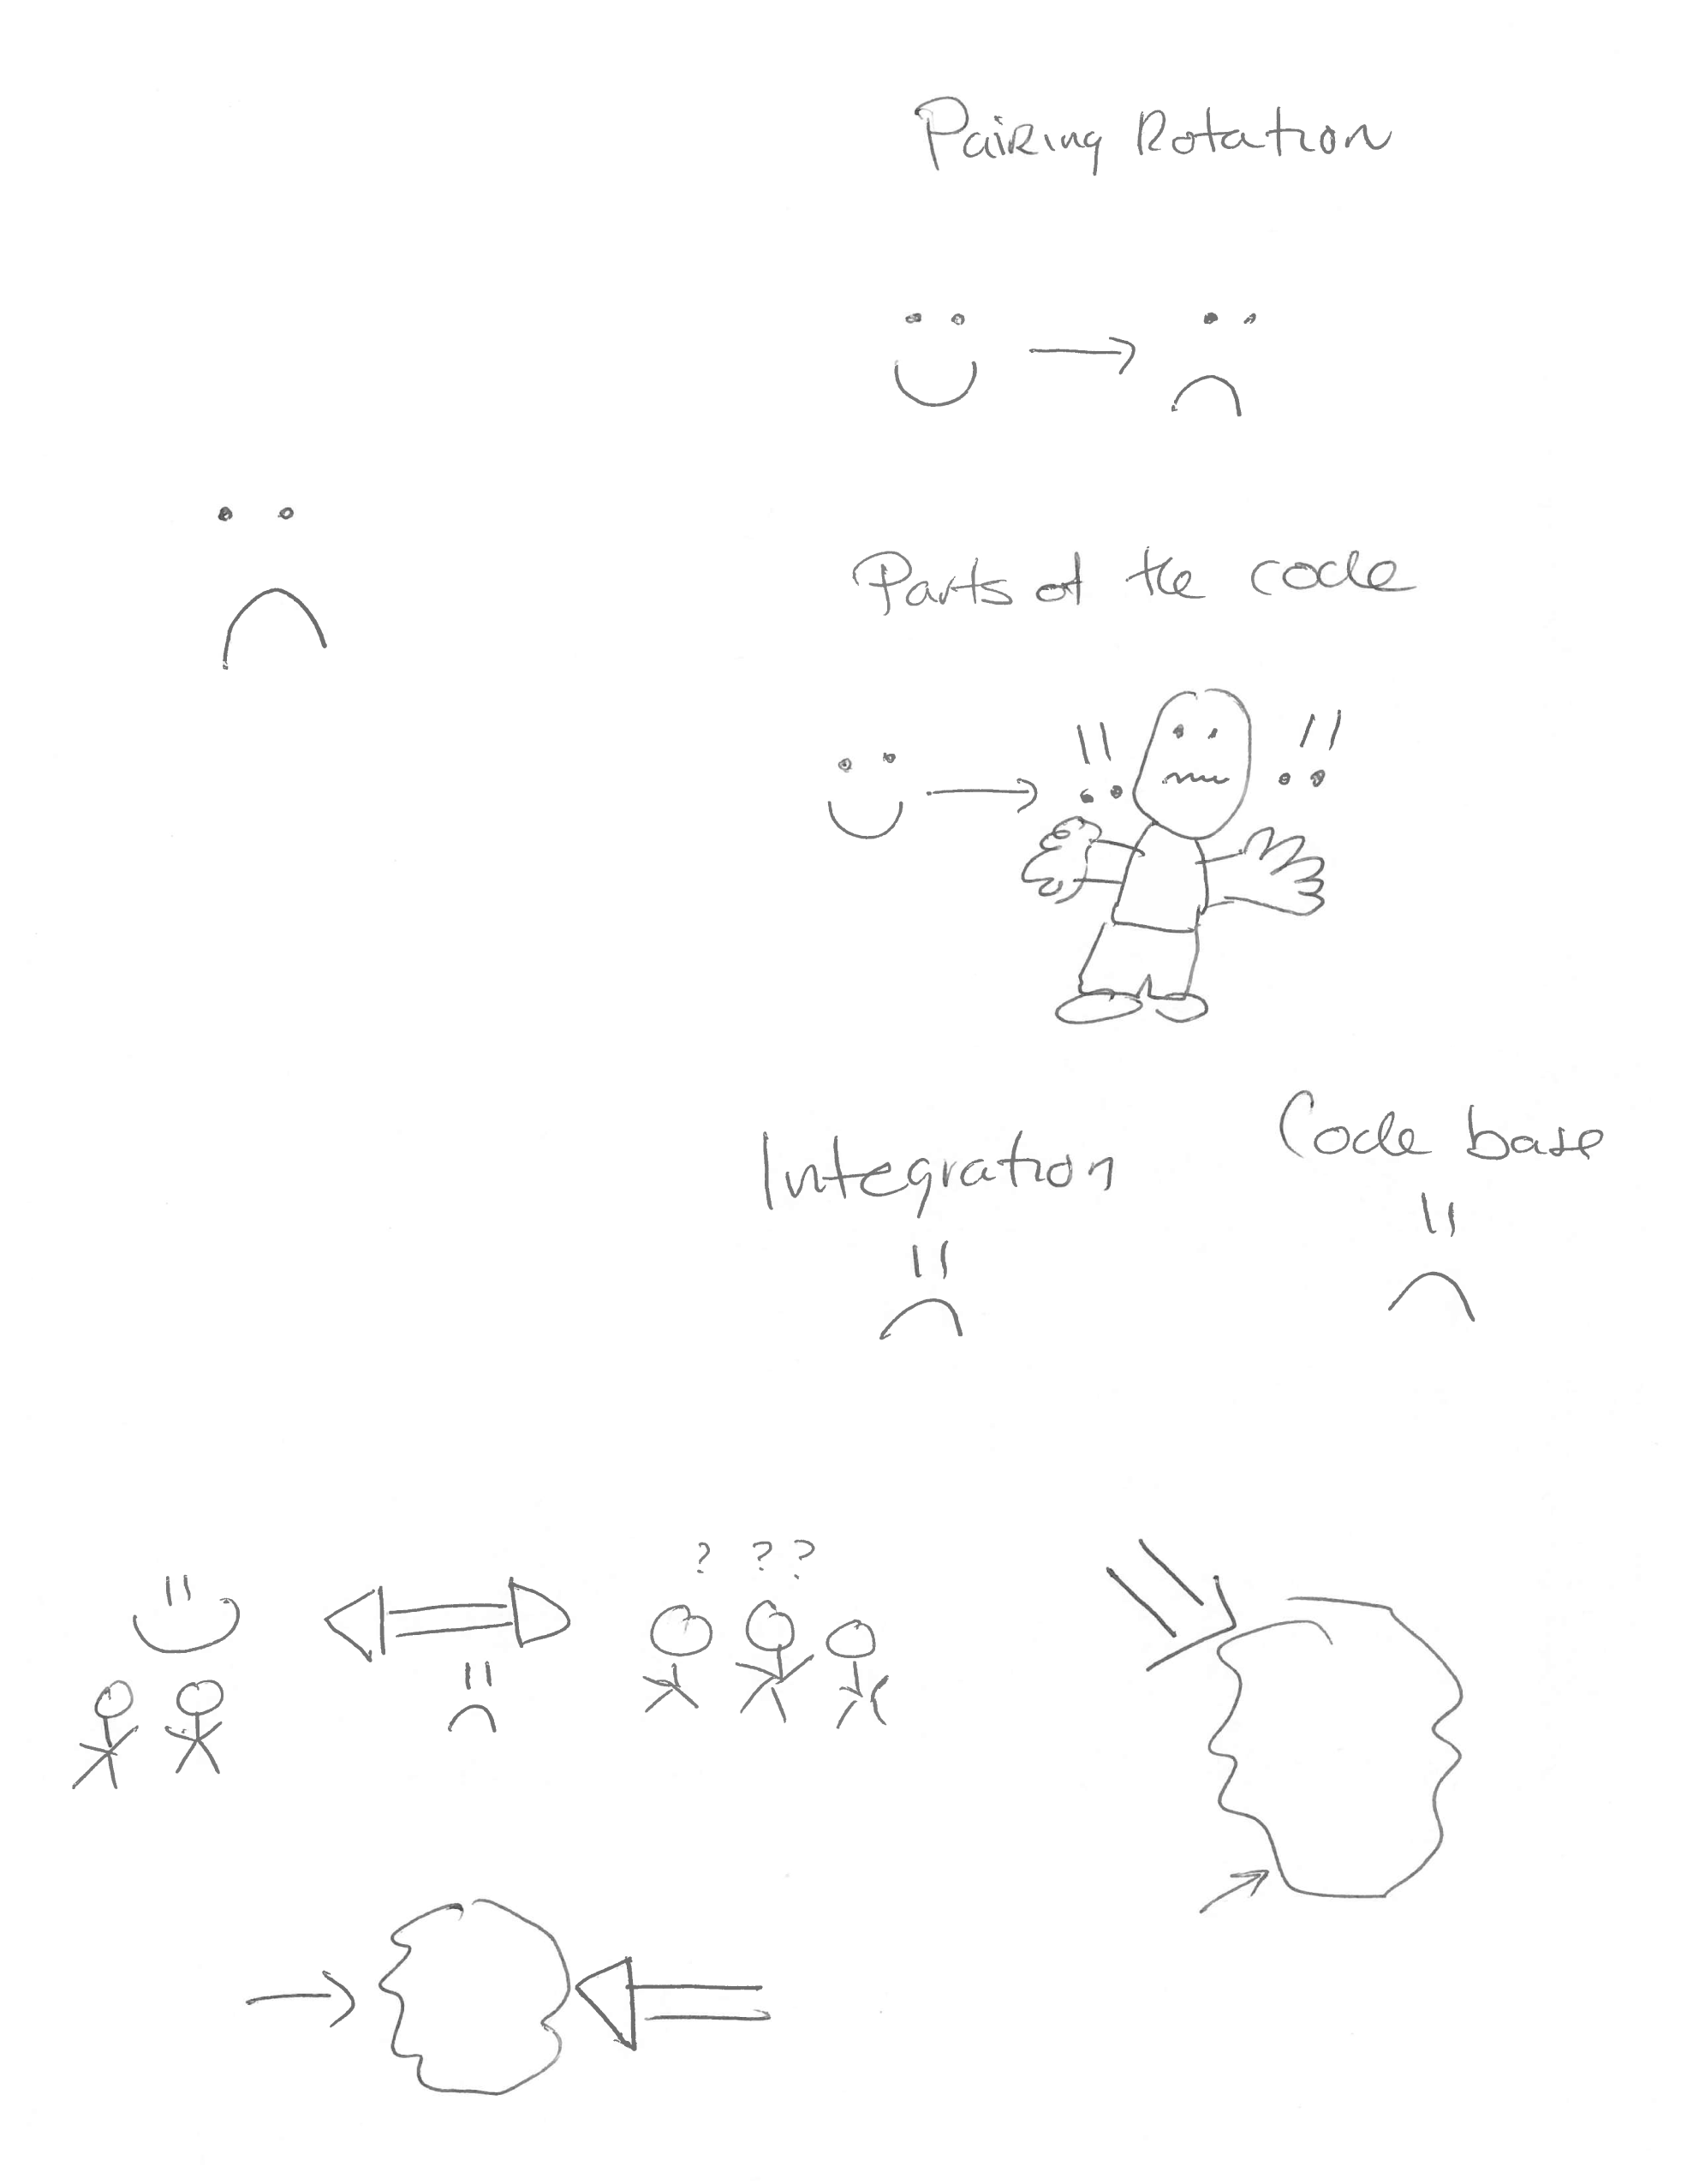
\includegraphics[width=6.5in]{interviews/drawings/2016_09_26_engineer2.png}
\caption{\quotes{Interview 32: Software Engineer's drawing for `How you feel or how you think about the code'}}
\end{figure}


\begin{figure}[H]
\centering
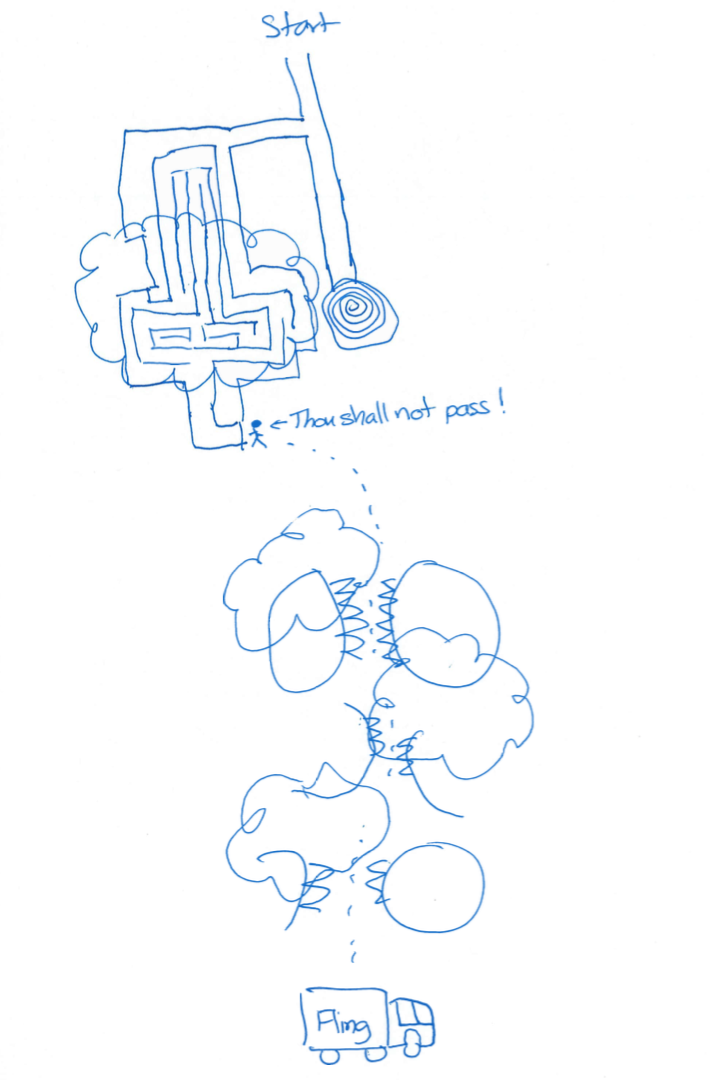
\includegraphics[width=5.6in]{interviews/drawings/2016_09_29.png}
\caption{\quotes{Interview 33: Software Engineer's drawing for `How you feel or how you think about the code'}}
\end{figure}
